\section{Diagramme d'Interaction}\label{sec:diagramme_interaction}
\begin{definition}[Diagramme d'Intéraction]
	Un diagramme d'intéraction (Interaction Overview Diagram) est un type de diagramme UML qui représente un diagramme d'activités au niveau global, liant les différents cas d'utilisation.
\end{definition}

\begin{figure}[H]
	\centering
\begin{subfigure}{0.45\textwidth}
	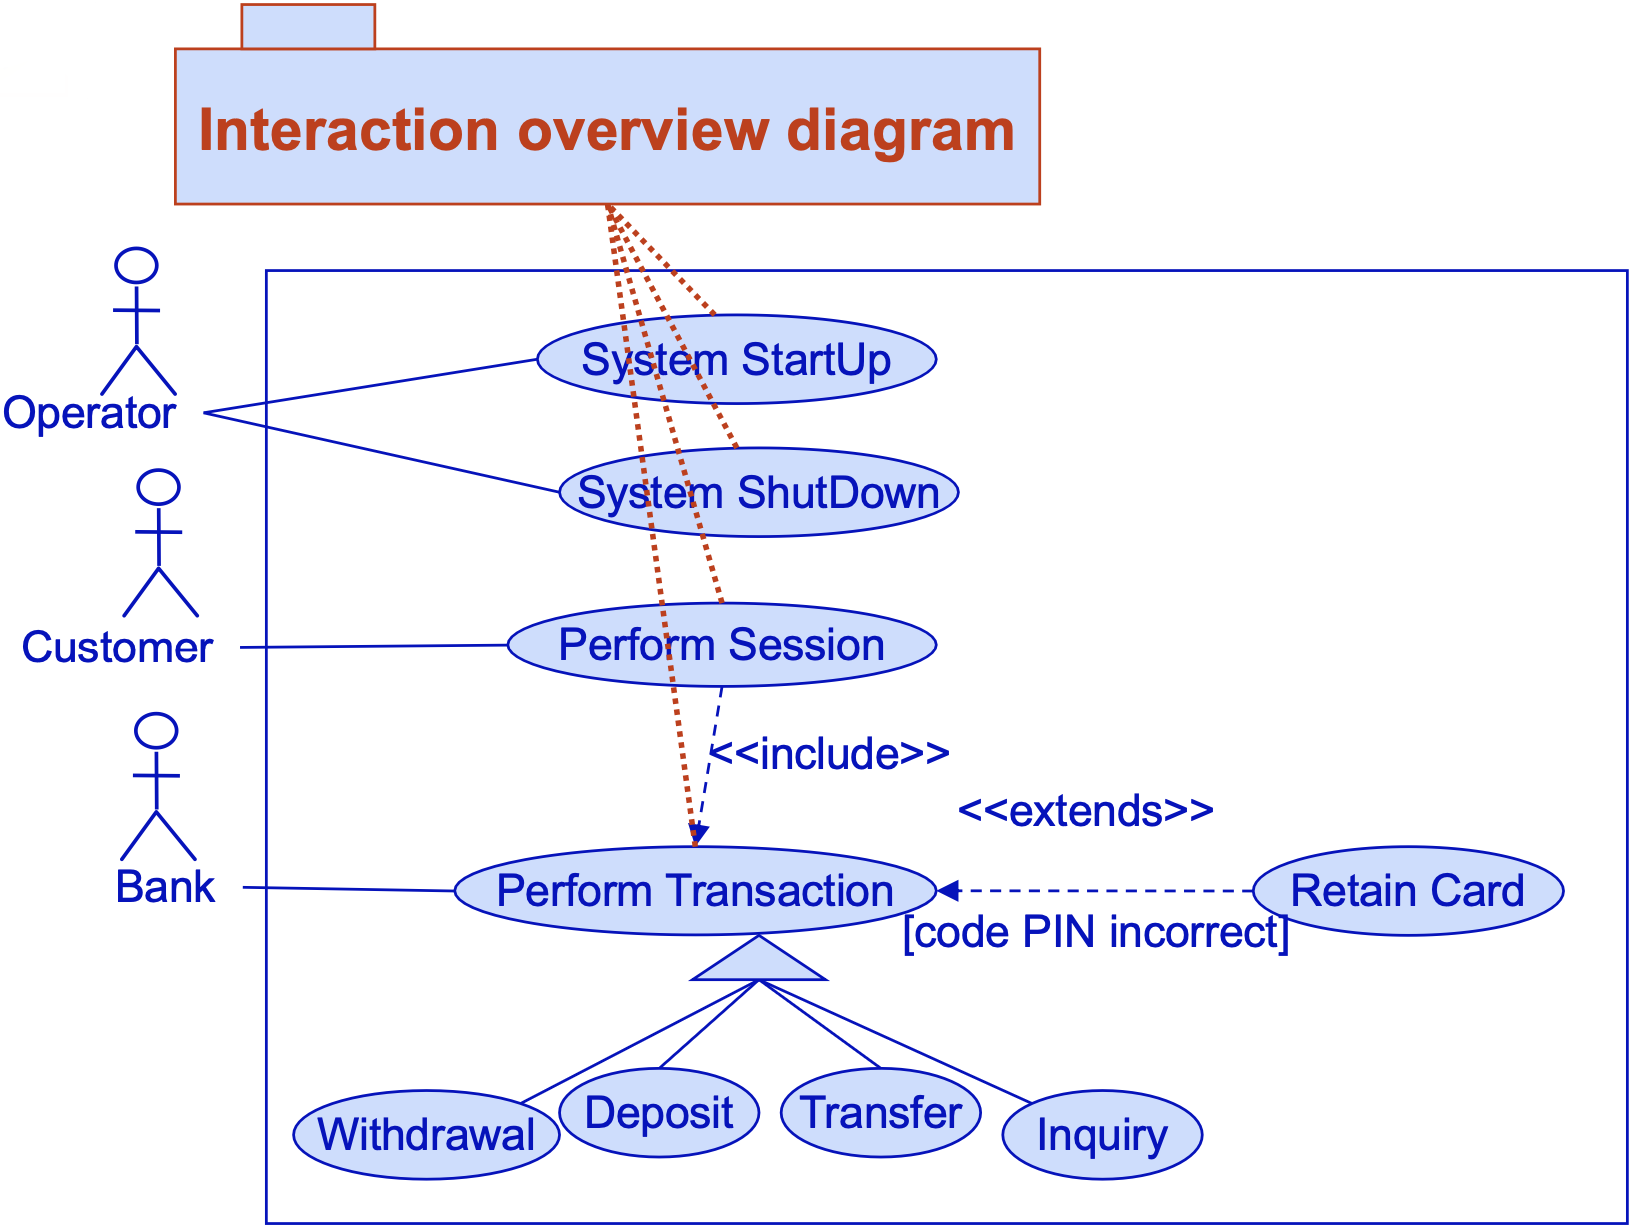
\includegraphics[width=\textwidth]{./Images/Diagrammes/diagram_interaction_ex_atm_usecase.png}
\end{subfigure}
\hfill
\begin{subfigure}{0.45\textwidth}
	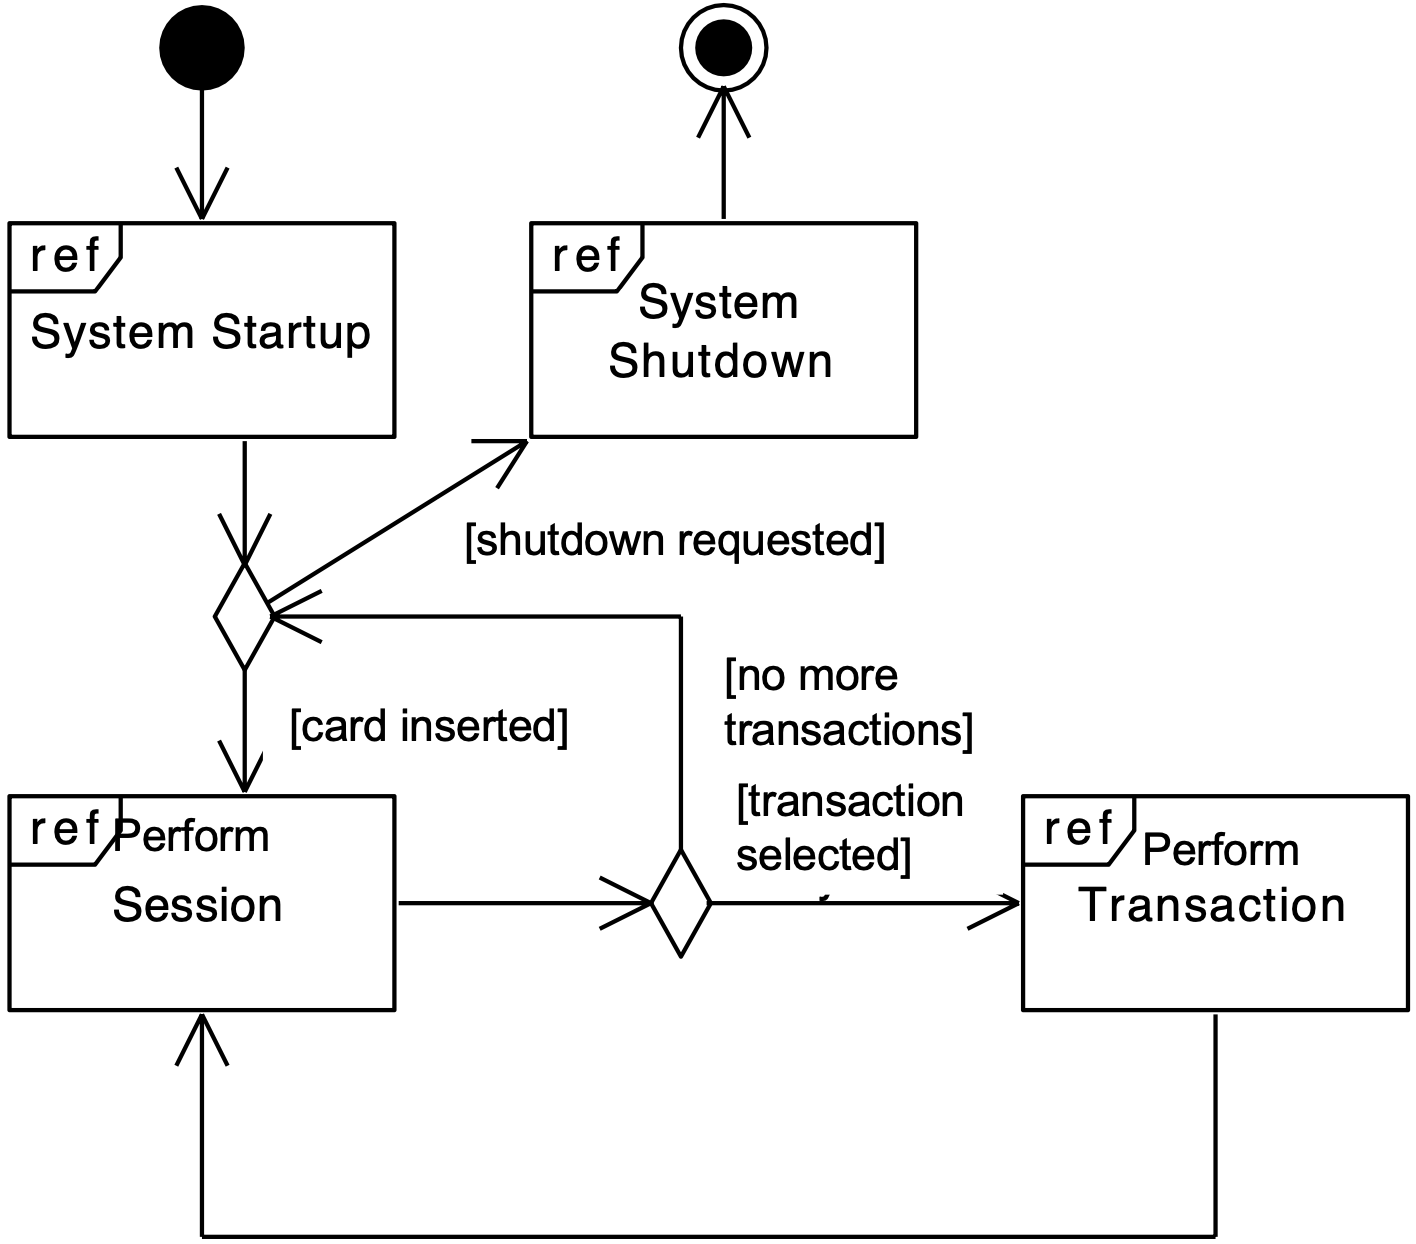
\includegraphics[width=\textwidth]{./Images/Diagrammes/diagram_interaction_ex_atm.png}
\end{subfigure}
\caption{Diagramme de Cas d'Utilisation vers Diagramme d'Intéraction}
\end{figure}